\documentclass[utf8]{gradu3}
% Jos työ on kandidaatintutkielma eikä pro gradu, käytä ylläolevan asemesta
%\documentclass[utf8,bachelor]{gradu3}
% Jos kirjoitat englanniksi, käytä ylläolevan asemesta
%\documentclass[utf8,english]{gradu3}
% tai
%\documentclass[utf8,bachelor,english]{gradu3}

\usepackage{graphicx} % kuvien mukaan ottamista varten
\graphicspath{ {./kuvat/} }

\usepackage{amsmath} % hyödyllinen jos tekstisi sisältää matikkaa,
                     % ei pakollinen

\usepackage{booktabs} % hyvä kauniiden taulukoiden tekemiseen

% HUOM! Tämän tulee olla viimeinen \usepackage koko dokumentissa!
\usepackage[bookmarksopen,bookmarksnumbered,linktocpage]{hyperref}

\addbibresource{gradu.bib} % Lähdetietokannan tiedostonimi

\begin{document}

\title{Äänipalautetyökalun suunnittelu, toteutus ja evaluointi}
\translatedtitle{Tool for giving recorded audio feedback in e-education}
\studyline{Ohjelmistotekniikka}
\avainsanat{%
  äänipalaute, raf, verkko-opetus, oppimisympäristö
  }
\keywords{recorded audio feedback, raf, e-education, e-education environment}
\tiivistelma{%
Tässä tutkielmassa arvioidaan voidaanko verkko-opetuksessa käytettävää äänipalautteen antamista helpottaa.
}
\abstract{%
  This Masters thesis is aimed at assessing whether the use of recorded audio feedback for online teaching can be facilitated.
}

\author{Erkko Mäkinen}
\contactinformation{\texttt{erkko.e.makinen@student.jyu.fi}}
% jos useita tekijöitä, anna useampi \author-komento
\supervisor{Anneli Heimbürger ja Ville Isomöttönen}
% jos useita ohjaajia, anna useampi \supervisor-komento

%\type{Tietotekniikan pro gradu -tutkielma} % et tarvitse tätä riviä tutkielmassa!

\maketitle


\begin{thetermlist}
\item[RAF] Recorded audio feedback \parencite[ks.][]{using}. 
\end{thetermlist}

\mainmatter

\chapter{Johdanto}

Palautteen antaminen opiskelijoille on erittäin tärkeää heidän oppimisensa kannalta, jotta he tietävät missä he ovat suoriutuneet hyvin ja missä heillä olisi vielä kehittämisen varaa. Palautteen antamiseen on useita erilaisia menetelmiä, joista kullakin on omat hyvät ja huonot puolensa. Äänipalautteen (engl. Recorded Audio Feedback, RAF) antaminen on yleistynyt lähivuosina, erityisesti verkko-oppimisen parissa, jossa suoraa kontaktia opettajaan tai muihin opiskelijoihin ei välttämättä ole ollenkaan. Opiskelun muututtua yhä teknologia-avusteisemmaksi, on tilanteeseen sopeuduttava myös palautteen antamisen laadun ja siihen liittyvien käytänteiden saralla \parencite[][]{cavanaugh2014}.

Tähän astisten tutkimusten perusteella voidaan sanoa, että äänipalaute koetaan positiivisena, vaikka siihen liittyykin tiettyjä haasteita. Äänipalautetta pystytään antamaan nopeasti, se on tekstimuotoista selkeämpää ja eroavaisuudet äänensävyn käytössä helpottaa palautteen tulkitsemista. Lisäksi palautteen kuuleminen lukemisen sijaan tuntuu henkilökohtaisemmalta, jolla taas on positiivisia vaikutuksia oppimiseen \parencite[][]{moderating}. Opiskelijoiden mukaan äänipalaute tukee oppimista parhaiten siten, että palautteen pääkohdat ovat kirjattu tekstimuotoisena ja tarkennukset niitä koskien äänipalautteena \parencite[][]{using}.

Vaikka äänipalautteella on tutkittu olevan selkeitä etuja etenkin verkko-opetuksessa, niin sen käyttämiseen voi olla iso kynnys johtuen siitä, että erityisesti sen antamiseen suunnattuja työkaluja on rajallisesti saatavilla ja niissä on vielä kehittämisen varaa. Nauhoitus ja editointi onnistuu useilla työkaluilla, mutta niiden opetteleminen ja käyttäminen voi olla haastavaa ja aikaavievää. Tällainen tekninen alkukömpelyys voi vaikuttaa siihen, kuinka äänipalautteen antaminen koetaan \parencite[][]{cavanaugh2014}.

Tässä tutkielmassa käydään läpi tämänhetkisiä haasteita liittyen äänipalautteen antamiseen ja niiden pohjalta luodaan alustariippumaton ja responsiivinen web-sovellus, jossa erityisesti helppokäyttöisyys on otettu huomioon. Ohjelmaa testataan siinä vaiheessa tutkimusta, kun se on mielekästä ja selvitetään tekeekö se äänipalautteen antamisesta helpompaa ja miellyttävämpää.

\chapter{Palaute}
\subsection{Millaista on hyvä palaute?}
\subsection{Formatiivinen palaute}
\subsection{Summatiivinen palaute}

%

\chapter{Äänipalaute}

\section{Hyvät ja huonot puolet}

\section{Äänipalautteen antaminen}


%

\chapter{Tutkimusmenetelmä}

Tämä Pro Gradu -tutkielman tutkimusmenetelmä pohjautuu suunnittelututkimukseen (engl. \textit{design science}), joka on käytännönläheinen tutkimusparadigma, jossa tarkoituksena on luoda artefakteja, ratkaisemaan erilaisia reaalimaailman ongelmia \parencite[][]{hevner2004}. Artefaktit voidaan määritelmältään jakaa neljään eri kategoriaan: konstruktioihin, malleihin, menetelmiin ja instansseihin \parencite[][]{hevner2004}. Tässä tutkimuksessa toteutettava artefakti, eli äänipalautetyökalu, luokitellaan instanssiksi, sillä tarkoituksen on suunnitella ja kehittää prototyyppisovellus, jonka avulla pyritään selvittämään, voidaanko äänipalautteen antamista helpottaa opettajan näkökulmasta. Äänipalautteen antaminen on siis tutkittava ongelma, johon äänipalautetyökalun suunnittelulla ja toteutuksella pyritään löytämään ratkaisuja. Näistä ongelmista ja tavoitteista johdetut tutkimuskysymykset ovat:

\begin{itemize}
  \item Helpottaako äänipalautetyökalu äänipalautteen antamista?
  \item Muuttaako äänipalautetyökalun käyttö suhtautimista äänipalautteen antamiseen?
\end{itemize}

Suunnitteluun liittyvää tutkimusta on tehty jo pitkään useilla eri tieteenaloilla \parencite[][]{cross2001}, mutta tietotekniikan aikakausi on tuonut uusia suunnitteluun liittyviä haasteita, jotka vaativat uusia luovia ratkaisutapoja \parencite[][]{design}. Aikoinaan suunnittelututkimuksen katsottiin kuuluvan enemmän teknisten tieteenalojen piiriin, mutta 1990-luvun alussa sen merkitys reaalimaailman liiketoimintaongelmien ratkaisemisessa artefaktien avulla havaittiin tärkeäsi \parencite[][]{design}, sillä tietojärjestelmien ensisijainen tavoite on nimenomaan kasvattaa yrityksen tehokkuutta \parencite[][]{hevner2004}. Tämän tutkielman tavoite ei kuitenkaan ole liiketoiminnallisten etujen tavoitteleminen, vaan äänipalautteen antamista helpottavien innovaatioiden löytämisessä ja tutkimisessa.

Suunnittelututkimksen avulla pyritään luomaan innovaatioita, jotka määrittävät ideat, käytännöt, tekniset mahdollisuudet ja tuotteet, joita hyödyntämällä tietojärjestelmien analyysi, suunnittelu, toteutus ja käyttö voidaan suorittaa tehokkaasti \parencite[][]{hevner2004}. Suunnittelututkimuksella pyritään löytämään ratkaisuja viheliäisiin ongelmiin (engl. \textit{wicked problem}), joita Rittel ja Webber \parencite[][]{wicked} luonnehtivat seuraavanlaisesti: 

\begin{itemize}
  \item Epävakaat vaatimukset ja rajoitteet
  \item Monimutkaiset vuorovaikutukset ongelman alikomponenttien kanssa
  \item Luontainen joustavuus suunnitteluprosessien ja artefaktien suhteen
  \item Riippuvuus ihmisen kognitiivisista kyvyistä tehokkaan ratkaisun saavuttamiseksi
  \item Riippuvuus ihmisen sosiaalisista kyvyistä tehokkaan ratkaisun saavuttamiseksi
\end{itemize}

Äänipalautetyökalun suunnittelu ja toteutus voidaan luokitella viheliääksi ongelmaksi, sillä siinä on samoja piirteitä kuin edellä mainitussa listauksessa. Työkalun vaatimukset ja rajoitteet olivat alussa epäselvät, sillä tarkoituksena on alunperin lähteä selvittämään, voidaanko ääniapalautteen antamista helpottaa tarkoitukseen suunnitellun työkalun avulla. Tämä epätietietoisuus myös vaikuttaa siihen, että artefaktin suunnittelu ja toteutus muovaantuu prosessin edetessä ja ongelmanratkaisu vaatii luovaa ajattelua. Lisäksi tutkielman ohjaajien ja muiden työkalun evaluointiin osallistuvien henkilöiden kokemuksella, näkemyksillä ja palautteilla on erittäin suuri merkitys artefaktin suunnittelu- ja toteutus -ratkaisuihin.

%

\section{Suunnittelututkimuksen syklit}

Suunnittelututkimuksen toteuttamiseen sisältyy on kolme oleellista sykliä: relevanssisykli, suunnittelusykli ja täsmällisyyssykli \parencite[][]{cycles}. Näitä syklejä toistetaan iteratiivisesti tutkimuksen lävitse, kunnes artefaktin osalta päädytään haluttuun lopputulokseen. Kuviossa ~\ref{fig:dsr} on esitetty suunnittelutukimuksen toteutukseen kuuluvat komponentit, joista syklit ovat korostettu sinisellä värillä. Kuvio pohjautuu Hevnerin vuonna 2004 \parencite[][]{hevner2004} laatimaan viitekehykseen, mutta kyseinen Hevnerin vuonna 2007 \parencite[][]{cycles} laatima kuvio keskittyy suunnittelutukimukseen liittyviin sykleihin. Seuraavissa alaluvuissa käsitellään kunkin kolmen syklin toteuttamista, merkityksiä ja ominaisuuksia, jotta voidaan ymmärtää miten suunnittelututkimus käytännössä toteutetaan. Lisäksi kutakin sykliä käsitellään tämän tutkimuksen näkökulmasta.

\begin{figure}[h]\centering
  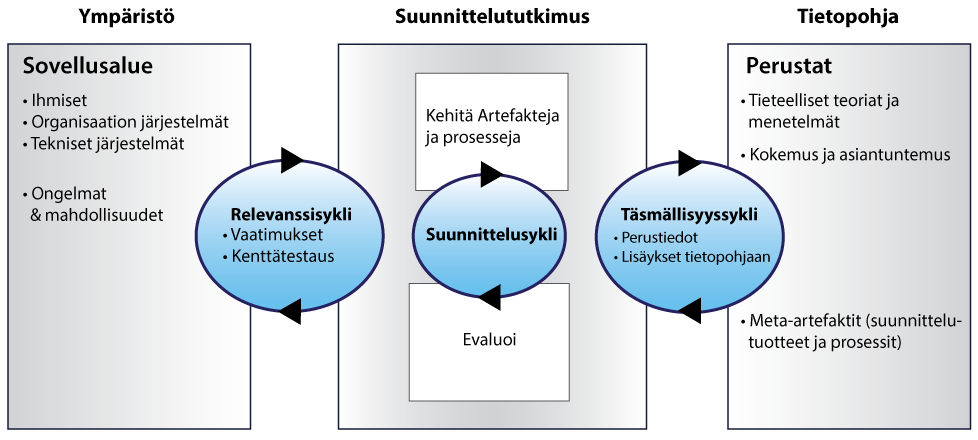
\includegraphics[height=7cm,keepaspectratio]{DSR}
  \caption[]{Suunnittelututkimuksen syklit}
  \label{fig:dsr}
\end{figure}

\subsection{Relevanssisykli}

Relevanssisykli on suunnittelututkimuksen aloittava sykli, joka määrittää sovellusalueen kontekstin tutkimukselle. Sovellusalue koostuu ihmisistä, organisaatiojärjestelmistä ja teknisistä järjestelmistä, jotka toimivat yhdessä tietyn tavoitteen saavuttamiseksi. Suunnittelututkimuksessa on oleellista löytää sovellusalueelta ongelmia tai mahdollisuuksia, joiden pohjalta lähdetään kehittämään niihin erilaisia ratkaisuja artefaktien avulla. Relevanssisykli määrittää ympäristön kautta suunnittelututkimukselle vaatimukset sekä hyväksymiskriteerit tutkimustulosten evaluoinnille. Oleelliset kysymykset ovat: helpottaako artefakti ympäristöään jollain tavalla, ja kuinka tämä parannus voidaan mitata \parencite[][]{cycles}?

Relevanssin toinen merkittävä osa on artefaktin kenttätestaus, joka voidaan suorittaa monin eri tavoin. Sen tarkoituksena on selvittää, täyttääkö artefakti sille määrätyt vaatimukset, ja tuoko se sitä kautta jonkin asteisia parannuksia ympäristöönsä. On myös mahdollista, että vaatimukset ovat alusta alkaen olleet väärät, jolloin ne täytyy uudelleenmäärittää. Suunnittelutukimuksen edetessä tulokset määrittävät sen, vaatiiko tutkimus ylimääräisiä relevanssisyklejä \parencite[][]{cycles}.

Tämän tutkimuksen sovellusalue koostuu yliopistosta organisaationa, opettajista sekä järjestelmistä, joita hyödynnetään äänipalautteen antamisessa. Ensimmäisen relevanssisyklin tärkein tavoite on selvittää, miten opettajat suhtautuvat äänipalautteen antamiseen, millaisia työkaluja he käyttävät sekä millä keinoin äänipalautteen antamista voidaan helpottaa. Relevanssisyklin erityisen tärkeä osa on ongelmien tai mahdollisuuksien löytäminen, jotka tämän tutkimuksen kohdalla saivat alkuunsa Heimburgerin, Isomöttösen ym. \parencite[][]{academics} tekemän tutkimuksen kautta. Tutkimuksessa tuli esille tiettyjä äänipalautteen antamiseen liittyviä ongelmia ja ideoita äänipalautteen antamiseen tarkoitetusta työkalusta, joiden pohjalta tässä suunnittelututkimuksessa lähdetään etenemään.

Kenttätestaus suoritetaan tutkimuksessa kehitettävän prototyyppisovelluksen käyttäjätestaamisella ja evaluoinnilla. Evaluoinnin suorittavat neljä opettajaa, joilla on jo aiempaa kokemusta äänipalautteen antamisesta. Kenttätestauksen suoritukseen osallistuvat tämän tutkielman ohjaajat Anneli Heimburger ja Ville Isomöttönen sekä kaksi muuta yliopistossa työskentelevää opettajaa Paavo Nieminen sekä Harri Keto. Evaluointia käsitellään tarkemmin luvussa X. 

\subsection{täsmällisyyssykli}

Täsmällisyyssyklin tarkoituksena on tuoda tutkimukseen aiempaa tietämystä aihealueeseen liittyen, jotta voidaan varmistua siitä, että toteutettavan suunnittelututkimuksen tulokset ovat innovaatiivisia. Suunnittelututkimus perustuu useimmiten tieteellisiin teorioihin, teknisiin menetelmiin sekä kokemuksiin ja asiantuntijuuteen, jotka määrittävät sovellusalueen sen hetkisen tilan. Lisäksi tietopohjaan kuuluuvat sovellusalueella jo käytössä olevat artefaktit ja prosessit \parencite[][]{cycles}.

Sopivien teorioiden ja menetelmien löytäminen artefaktin kehittämisen ja evaluoinnin tueksi on suunnittelututkimuksen toteuttajien yksi perustavanlaatuisista tehtävistä. On kuitenkin epärealistista ja alalle haitallista odottaa, että kaikki suunnittelututkimuksen osa-alueet perustuvat tiettyihin teorioihin. Suotuisampaa on tunnistaa useita idoiden lähteitä, jotka luovat pohjan suunnittelututkimuksen toteuttamiselle \parencite[][]{cycles}.

Jos suunnittelutukimuksen tulokset ovat innovatiivisia, ne tuovat eri asteisia lisäyksiä sovellusalueen tietopohjaan. Muutoksen voivat liittyä teorioihin, menetelmiin, meta-artefakteihin tai kokemuksiin, jotka on saavutettu tutkimuksen ja kenttätestauksen toteuttamisen yhteydessä \parencite[][]{cycles}.

Tämän suunnittelututkimuksen tietopohja pohjautuu opettajien kokemuksiin ja näkemyksiin äänipalautteen antamisesta, käyttöliittymäsuunnittelussa hyödynnettäviin käytettävyysperiaatteisiin sekä erilaisten nauhoitus- ja äänipalautetyökalujen tämänhetkiseen tilaan.  Kuten jo aiemmin on mainittu, niin tämä suunnittelututkimus sai alkunsa tutkimuksesta, joka käsittelee äänipalautteen antamista opettajien näkökulmasta. Tutkimuksessa tuli esille tietynlaisia haasteita äänipalautteen antamiseen liittyen, sekä ideoita äänipalautteen antamiseen suunnatusta työkalusta. Jo olemassa olevien nauhoitus- ja äänipalautetyökalujen tutkimisen pohjalta voidaan todeta, että työkalut eivät ole täysin soveltuvia äänipalautteen antamiseen ja sitä kautta niissä on parantamisen varaa. Esimerkiksi useimmat äänipalautteen antamiseen suunnatut työkalut ovat kaupallisia, joten niiden käyttö opetuksessa on lähes aina poissuljettua. Jo tämän tutkimuksen alkuvaiheilla oli selkeää, että äänitteen väliin tulisi pystyä nauhoittamaan uusi äänite mahdollisimman helposti. Monissa äänitystyökaluissa tämä onnistuu, mutta se vaatii useita peräkkäisiä toimintoja. Lisäksi työkalut sisältävät runsaasti sellaisia toimintoja, jotka ovat äänipalautteen antamisessa tarpeettomia. Pelkästään näiden tietojen pohjalta saadaan varmuus siihen, että suunnittelututkimuksessa kehitetään jotain uutta ja innovatiivista.

Käyttöliittymän suunnittelu on erittäin tärkeää, jotta työkalu olisi käytettävyydeltään mahdollisimman hyvä. Suunnittelun apuna tutkimuksessa käytetään kahta toisistaan eroavaa käytettävyysperiaatteiden joukkoa. Nielsenin heuristiikat tarjoavat yleisiä käytettävyyteen liittyviä ohjenuoria kun taas Gestaltin hahmolait keskittyvät käyttöliittymän visuaalisuuteen ihmisaivojen hahmottelukyvyn kautta. Suunnittelussa hyödynnettyjä käytettävyysperiaatteita käsitellään tarkemmin luvussa X.

Äänipalautetyökalun evaluointi suoritetaan hyvin vapaamuotoisena käyttäjäkyselynä, joka suoritetaan kahteen kertaan tutkimuksen eri vaiheissa. Kyselyn tärkein tavoite on saada selville helpottiko äänipalautetyökalu äänipalautteen antamista tai siihen suhtautumista. Lisäksi evaluointiin kuuluu työkalun tarkoituksenmukaisuuden, perustoimintojen sekä käytettävyyden arviointi. Evaluointi on täysin laadullinen, sillä edellä mainittujen ominaisuuksien arvioiminen olisi määrällisesti haastavaa, erityisesti kun kyseessä on keskeneräinen prototyyppisovellus. Äänipalautetyökalun evaluointia käsitellään tarkemmin luvussa X.

\subsection{Suunnittelusykli}

Suunnittelututkimuksen tärkein sykli on suunnittelusykli, joka koostuu artefaktin suunnittelusta ja evaluoinnista. Tarkoituksena on luoda erilaisia suunnittelutyön tuotoksia, arvioida niitä, ja tarkistaa vastaavatko ne relevanssisyklissä määritettyjä vaatimuksia. Artefaktien suunnittelu ja evaluointi toteutetaan täsmällisyyssyklissä määritettyjä teorioita ja mentelmiä hyödyntäen. Suunnittelusyklissä tapahtuu suurin osa suunnittelututkimuksen työstä, ja tästä syystä iteraatioita on tiheämmin kuin relevanssisyklissä tai täsmällisyyssyklissä, jotka luovat pohjan suunnittelusyklissä toteutettaville toimenpiteille \parencite[][]{cycles}.

Suunnuittelusyklissä on tärkeää jakaa vaivannäkö tasaisesti sekä artefaktin kehittämiselle että evaluoinnille, sekä molempien toimintojen tulisi perustua relevanssisyklistä ja täsmällisyyssyklissä määritettyihin teorioihin tai menetelmiin. Suunnittelusykliä joudutaan lähes aina iteroimaan useita kertoja, ennen kuin sen tuloksia voidaan hyödyntää relevanssi ja täsmällisyyssyklissä \parencite[][]{cycles}.

Tässä tutkimuksessa suunnittelusyklien määrä joudutaan rajaamaan kahteen iteraatioon, jotta tutkimuksen laajuus vastaisi tyypillistä pro gradu -tutkielmaa. Ensimmäisen iteraation tavoitteena on kehittää prototyyppi sellaiseen pisteeseen, että äänipalautteen äänittäminen ja editointi olisi mahdollista. Tämä siis tarkoittaa sitä, että työkalun käyttöliittymä, perustoiminnot ja äänileikenäkymä on toteutettu ja testattu tiettyyn pisteeseen. Evaluoinnin tärkein tavoite on löytää äänipalautetyökalun hyvät ja huonot suunnitteluratkaisut, sekä selvittää kaipaako työkalu vielä ylimääräisiä toiminnallisuuksia. Ensimmäisen iteraation suorittavat Anneli Heimburger ja Ville Isomöttönen, jotka toimivat tämän tutkielman ohjaajina. Kaksi muuta koehenkilöä osallistuvat ohjaajien lisäksi vasta toiseen iteraatioon, jossa artefaktiin on tehty muutoksia ensimmäisen iteraation pohjalta.

Näiden kahden suunnittelusyklin lisäksi äänipalautetyökalun kehittäminen tapahtuu useissa pienemmissä sykleissä, jotka muistuttavat varsinaista suunnittelusykliä. Artefaktin suunnitteluratkaisuista neuvotellaan palavereissa ohjaajien kanssa, joilla on kokemusta äänipalautteen antamisesta. Kun suunnitellut ominaisuudet on toteutettu, arvioidaan onko työkalun suunta oikea, ja sovitaan jatkotoimenpiteistä seuraavaa palaveria varten. Tällä syklillä on yhtäläisyyksiä myös relevanssisyklin kanssa, jossa mm. määritellään artefaktin vaatimuksia.

\section{Artefaktin evaluointi}

\subsection{evaluoinnin kriteerit}
\label{kriteerit}

Artefaktin evaluointi on suunnittelututkimuksen merkittävä osa, jossa arvioidaan tietyin menetelmin, täyttääkö artefakti sille määrätyt kriteerit. Suunnittelututkimuksen alkuvaiheilla on tärkeä määrittää mihin objektiin evaluointi kohdistuu ja mitkä ovat evaluoinnin kriteerit, sekä määrittää kuinka artefakti evaluoidaan ja mitä menetelmiä siinä hyödynnetään \parencite[][]{evaluation}. 

Simonin \parencite[][]{simon1996} mukaan suunnitteluartefaktit voidaan mieltää järjestelmiksi. Myös muualla suunnittelututkimukseen liittyvässä kirjallisuudessa artefakteista puhutaan järjestelminä, joten evaluointikriteerien määrittelyssä voidaan hyödyntää systeemiteoriaa \parencite[][]{evaluation}. Systeemiteorian mukaan järjestelmä on suhteessa toisiinsa olevien osien summa, joka luo uusia ominaisuuksia, ja jolla on jokinlainen tavoite \parencite[][]{skyttner}. Järjestelmän kanonisen muodon mukaan järjestelmällä on viisi ulottuvuutta: tavoite, ympäristö, rakenne, aktiivisuus ja evoluutio \parencite[][]{modeling, systemic}.

Edellä mainittuja järjestelmän ulottuvuuksia voidaan hyödyntää artefaktin evaluointikriteerien määrittämisessä.  Prat, Comyn-Wattiau ja Akoka \parencite[][]{evaluation} ovat laatineet evaluaointikriteerien hierarkian, johon on kerätty kirjallisuudessa esiintyviä evaluointikriteerejä. Löydetyt kriteerit on jaoteltu järjestelmän ulottuvuuksien mukaan omiksi ryhmikseen ja osa evaluointikriteereistä on jaettu vielä useampiin alakriteereihin. Evaluointikriteerien hierarkia on esitetty kuviossa ~\ref{fig:evaluointikriteerit}.

\begin{figure}[h]\centering
  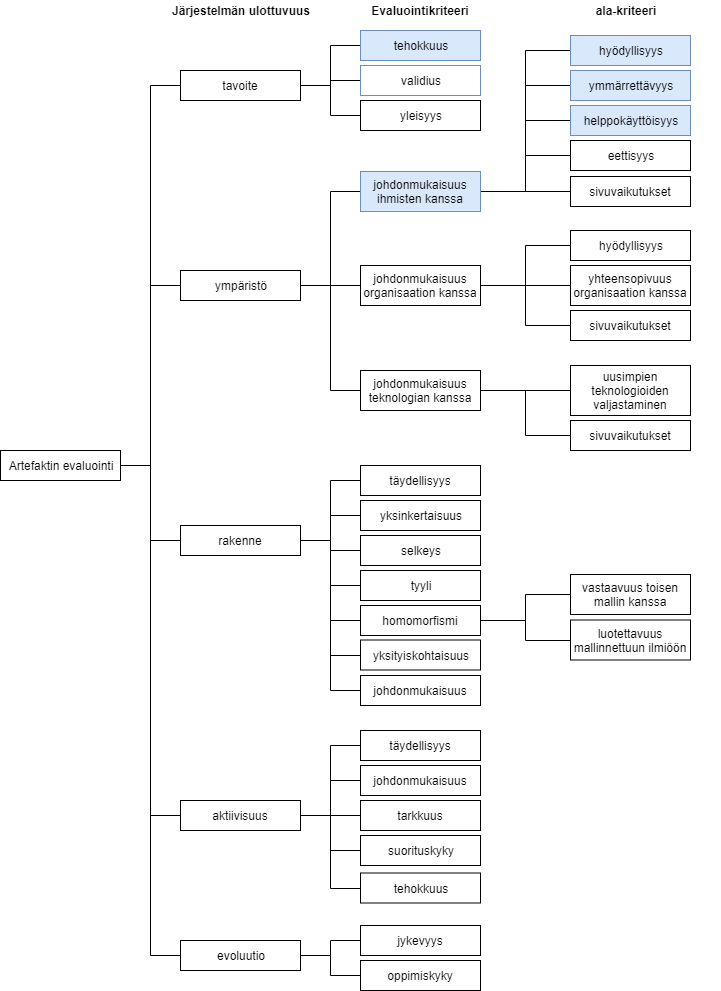
\includegraphics[width=\textwidth,height=\textheight,keepaspectratio]{evaluointikriteerit}
  \caption[]{Evaluointikriteerien hierarkia Pratin, Comyn-Wattiaun ja Akokan \parencite[][]{evaluation} laatimaa kuviota mukaillen. Äänipalautetyökalun evaluoinnin kannalta tärkeimmät evaluointikriteerit on korostettu sinisellä värillä.}
  \label{fig:evaluointikriteerit}
\end{figure}

Järjestelmän ulottuvuuksista tavoitteen alle on luokiteltu seuraavat evaluointikriteerit:  tehokkuus, pätevyys sekä yleisyys. Tehokkuudella mitataan sitä, kuinka hyvin artefakti onnistuu sille määrätyn tavoitteen saavuttamisessa, kun taas pätevyydellä mitataan, toimiiko artefakti oikealla tavalla. Yleisyydellä tarkoitetaan artefaktin tavoitteen laajutta \parencite[][]{evaluation}.

Artefaktin ympäristö koostuu ihmisistä, organisaatioista ja teknologiasta \parencite[][]{hevner2004}. Evaluointikriteereiksi on tästä johtuen määritelty kunkin edellä mainitun osan johdonmukaisuus, jolla tarkoitetaan kunkin osan, tai niistä muodostuvan kokonaisuuden yhteensopivuutta. Nämä evaluointikriteerit on vielä jaoteltu useampiin alakriteereihin, joista sekä ihmisten ja organisaation johdonmukaisuuden alle kuuluva hyödyllisyys mittaa, kuinka laadukkaasti artefakti toimii käytännössä. Ihmisten johdonmukaisuuteen liittyvät muut alakriteerit ovat ymmärrettävyys, helppokäyttöisyys, eettisyys sekä sivuvaikutukset. Organisaation muut johdonmukaisuuden alakriteerit ovat artefaktin yhteensopivuus organisaation kanssa ja sen sivuvaikutukset. Teknologian johdonmukaisuuden alakriteerit ovat uusimpien teknologien valjastaminen ja sivuvaikutukset \parencite[][]{evaluation}.

Järjestelmän rakenteeseen liittyvät evaluointikriteerit ovat artefaktin täydellisyys, yksinkertaisuus, selkeys, tyyli, homomorfismi, yksityiskohtaisuus sekä johdonmukaisuus \parencite[][]{evaluation}. Tämä järjestelmän ulottuvuus liittyy artefakteista malleihin, menetelmiin ja rakennelmiin, joten kriteerejä ei käsitellä sen tarkemmin.

Järjestelmän ulottuvuuksista aktiivisuus liittyy artefaktin toimintaan, ja se sisältää seuraavat evaluointikriteerit: täydellisyys,  johdonmukaisuus, tarkkuus, suorituskyky sekä tehokkuus. Artefaktin toiminnan täydellisyys ja johdonmukaisuus liittyy sekä toiminnalliseen että rakenteelliseen näkökulmaan, ja toiminnan tarkkuus varmistaa sen, että artefaktin tulokset eivät ole ristiriidassa jo olemassa olevien kokeiden kanssa. Suorituskyvyllä tarkoitetaan toiminnan nopeutta tai suoritustehoa, ja tehokkuus mittaa toiminnan syötteiden ja ulostulon välistä suhdetta \parencite[][]{evaluation}.

Järjestelmän evoluutio pitää sisällään evaluaatiokriteereistä jykevyyden (engl. robustness) sekä oppimiskyvyn. Vakaudella tarkoitetaan artefaktin kykyä sopeutua ympäristön muutoksiin ja oppimiskyvyllä sen kykyä oppia asioita aiemmista kokemuksista sekä ympäristön reaktioista \parencite[][]{evaluation}.

Äänipalautetyökalun evaluoinnissa selkeästi tärkeimmät järjestelmän ulottuvuudet ovat tavoite ja ympäristö. Tavoite-ulottuvuuteen sisältyvistä evaluontikriteereistä huomioon otetaan tehokkuus, jolla mitataan sitä, kuinka tehokkaasti artefaktilla pystytään suorittamaan sille oleellinen tehtävä, sekä validius, joka koskee sitä, kuinka oikein artefakti toimii tämän tavoitteen saavuttamisessa. Tehokkuus on kriteereistä tärkein, sillä tutkimuksen tavoitteena on nimenomaan tutkia, voidaanko äänipalautteen antamista helpottaa siihen suunnitellun työkalun avulla. Validiutta tutkimalla tavoitteen saavuttamista voidaan mahdollisesti tehostaa entisestään, joten se on myös oleellinen evaluoinnin kriteereistä. Yleisyys on rajattu evaluointikriteereistä ulkopuolelle, sillä työkalun tavoite on selkeä ja rajattu.

Ympäristö-ulottuvuuden alle kuuluvista evaluointikriteereistä tutkimukseen otetaan johdonmukaisuus ihmisten kanssa, joka on myös yksi evaluoinnin tärkeimmistä kriteereistä. Se jakautuu useampaan alakriteeriin, joista evaluointiin otetaan mukaan hyödyllisyys, ymmärrettävyys ja helppokäyttöisyys. Nämä ovat tärkeitä artefaktin laatuattribuutteja, sillä ne liittyvät suurelta osin käyttäjäkokemukseen, joka taas vaikuttaa käyttäjän suhtautumiseen ja oppimiskynnykseen työkalua koskien. Johdonmukaisuus ihmisten kanssa -evaluointikriteeristä on rajattu ulos eettisyys ja sivuvaikutukset, joilla ei tässä tutkimuksessa ole merkitystä.

Suurin osa suunnittelututkimuksista keskittyy organisaation toiminnan tehostamiseen, mutta tämä tutkimus keskittyy poikkeuksellisesti enemmän ihmisten suhtautumiseen ja kokemuksiin artefaktiin liittyen. Sen lisäksi, koska evaluoitava artefakti on prototyyppi, niin evaluointikriteeri johdonmukaisuus organisaation kanssa rajataan evaluoinnin ulkopuolelle, mutta siihen liittyviä seikkoja voidaan mahdollisesti arvioida evaluoinnin tulosten perusteella välillisesti. 

Rakenteeseen, aktiivisuuteen ja evoluutioon liittyvät evaluointikriteerit voidaan rajata suoraan evaluoinnin ulkopuolelle, sillä evaluoinnin kohteena oleva artefakti on prototyyppi. Ne ovat yksityiskohtaisempia kriteerejä, jotka liittyvät vahvasti mm. viimeistelyyn, täydellisyyteen, suoritustehoon ja mukautuvuuteen, jota ei prototyypiltä voida vaatia. Äänipalautteen suunnittelussa ja toteutuksessa nämä seikat on myös jätetty lähes täysin huomiotta, sillä tarkoituksena on kahden tutkimusiteraation kautta saada selville työkalun toimivat ja ei-toimivat ratkaisut tavoitteeseen ja käyttäjäystävällisyyteen liittyen.

\subsection{Artefaktin evaluointimenetelmät}

Artefaktin evaluointi voidaan suorittaa useilla eri menetelmillä.  Prat, Comyn-Wattiau ja Akoka \parencite[][]{evaluation} ovat omassa suunnittelututkimuksessaan luoneet mallin, joka kuvaa evaluointimenetelmän erilaisia ominaisuuksia. He ovat jaotelleet evaluointimenetelmän kokonaisuudessaan viiteen eri komponenttiin, joita ovat evaluointikriteerit, evaluoinnin tyyppi, evaluoinnin taso, evaluoinnin suhteellisuus sekä toissijaiset osallistujat. Evaluoinnin kriteerit on käsitelty edellisessä alaluvussa \ref{kriteerit}. Evaluoinnin tyyppi jaotellaan joko määrälliseksi tai laadulliseksi, joista määrällinen tuottaa jonkin mitatun tai havaitun numeerisen arvon \parencite[][]{evaluation}. Evaluointi voi olla joko abstrakti- tai instanssi-tasoinen, joka riipuu evaluoitavan artefaktin ominaisuuksista. Instanssitasoinen evaluointi voidaan suorittaa, joko kuvitteellisten tai autenttisten tehtävänantojen kautta. Evaluointi voi olla suhteellisuudeltaan absoluuttinen, suhteessa samankaltaisiin artefakteihin tai suhteessa artefaktin puuttumiseen. Toissijaiset osallistujat taas ovat henkilöitä, jotka testaavat esimerkiksi artefaktin prototyyppiä \parencite[][]{evaluation}. Edellä mainituista evaluoinnin ominaisuuksista osa jakautuu vielä alaluokkiin.

Tässä tutkimuksessa suoritettava äänipalautetyökalun evaluointi on instanssitasoista, sillä abstraktin artefaktin sijaan evaluoinnin kohteena on prototyyppi äänipalautetyökalusta. Usein prototyyppiä evaluoidessa hyödynnetään toissijaisia osallistujia, mutta tämän tutkimuksen tapauksessa artefaktia evaluoivat ainoastaan ensisijaiset koehenkilöt. Ensimmäiseen iteraatioon osallistuu kaksi henkilöä, ja toiseen iteraatioon neljä henkilöä.

Molemmat evaluointikerroista suoritetaan lähes samalla tavalla, pieniä muutoksia lukuunottamatta. Koehenkilöille lähetetään sähköpostin välityksellä linkki äänipalautetyökaluun, sekä arviointilomakkeeseen, jossa heidän tulee vastata äänipalautetyökalua koskeviin kysymyksiin. Evaluoinnin ohjeistukset on kerrottu arviointilomakkeen alussa. Koehenkilöitä pyydetään aluksi käyttämään äänipalautetyökalua autenttisessa tilanteessa, jotta evaluoinnin tulokset olisivat mahdollisimman tarkkoja. Koehenkilöt voivat suorittaa testauksen, joko mobiililaitteella, tabletilla tai tietokoneella, sillä työkalun tarkoituksen on toimia joustavasti alustasta tai laitteesta riippumatta. Koekäytön jälkeen heitä pyydetään testaamaan jokaista työkalun perustoimintoja, joita annetun tehtävän aikana koehenkilö ei testannut. Nämä kaksi tehtävänantoa suoritettuaan koehenkilön tulee vastata lomakkeella esitettyihin kysymyksiin. Lomakkeella käyttäjän tulee arvioida, palveliko äänipalautetyökalu tarkoitustaan, helpottiko työkalu äänipalautteen antamista entuudestaan, tai muuttiko se suhtautumista äänipalautteen antamiseen. Sen lisäksi koehenkilön tulee arvioida työkalun perustoiminnallisuuksia, jos joitakin huomioita niihin liittyen ilmaantuu. Lomakkeen viimeisissä osioissa käyttäjällä on mahdollisuus tuoda vapaamuotoisesti ilmi työkaluun liittyviä huomioita ja kehitysideoita.

Evaluointi on suhteeltaan absoluuttinen, suhteessa muihin samankaltaisiin artefakteihin, sekä suhteessa vastaavanlaisten artefaktien puuttumiseen, joten se kattaa kaikki kolme osa-aluetta. Evaluoinnissa arvioidaan absoluuttisesti työkalun tarkoituksenmukaisuutta ja toiminnallisuutta, mutta lisäksi äänipalautteen antoa pyydetään vertaamaan koehenkilön aiempiin kokemuksiin. Toisaalta aivan vastaavanlaisia äänipalautteen antamiseen suunniteltuja artefakteja ei ole vielä kehitetty, joten vertaaminen tapahtuu esimerkiksi perinteisiä nauhoitusohjelmia vasten.

\begin{table}[t]
\caption{Yhteenveto evaluoinnista}
\begin{tabular}{|l|l|l|l|l|}
\hline
Kuvaus                                                                                                                                         & evaluointikriteerit                                                                                                                                                                             & \begin{tabular}[t]{@{}l@{}}evaluoinnin\\  tyyppi\end{tabular} & \begin{tabular}[t]{@{}l@{}}evaluoinnin\\ taso\end{tabular} & \begin{tabular}[t]{@{}l@{}}evaluoinnin \\ suhteellisuus\end{tabular}                                                                                  \\ \hline
\begin{tabular}[t]{@{}l@{}}Äänipalautetyökalun\\ tarkoituksenmukaisuuden, \\ käytettävyyden ja \\ toiminnallisuuden\\ evaluointi.\end{tabular} & \begin{tabular}[t]{@{}l@{}}Tavoite / tehokkuus\\ Tavoite / validius\\ \\ ympäristö / \\ johdonmukaisuus\\ ihmisten kanssa /\\ hyödyllisyys,\\ ymmärrettävyys, \\ helppokäyttöisyys\end{tabular} & Laadullinen                                                   & Instanssi                                                  & \begin{tabular}[t]{@{}l@{}}Absoluuttinen,\\ \\ suhteessa saman-\\ kaltaisiin\\ artefakteihin,\\ \\ suhteessa artefaktien \\ puuttumiseen\end{tabular} \\ \hline
\end{tabular}
\end{table}

\chapter{Työkalun suunnittelu ja toteutus}

Tässä luvussa käsitellään äänipalautetyökalu-prototyypin suunnittelua ja toteutusta eri näkökulmista. Aluksi läpikäydään työkalun tekniseen toteutukseen liittyviä seikkoja, jonka jälkeen käsitellään käyttöliittymän suunnitelua ohjaavia käytettävyyysperiaatteita sekä itse käyttöliittymää. Lopuksi esitetään työkalun perus- ja erikoistoiminnot, ja kuinka näihin toiminnallisuuksiin päädyttiin.

Työkalu suunniteltiin pääasiassa yhteistyössä pro gradu -ohjaajien kanssa, joilla molemmilla on kokemusta äänipalautteen antamisesta. He ovat myös olleet osallisina tutkimuksessa, jossa selvitettiin akateemikkojen suhtautumista äänipalautteen antamiseen. Tutkimuksessa kolmella neljästä koehenkilöstä heräsi ideoita työkalusta, jolla äänipalautetta voisi antaa, editoida, hallita ja arkistoida \parencite[][]{academics}. Edellä mainitun tutkimuksen, sekä ohjaajien omien kokemusten ja näkemysten pohjalta äänipalautetyökalun suunnittelu ja toteutus päätettiin aloittaa.

\section{Tekniset toteutusratkaisut}

Äänipalautetyökalun yksi tärkeimmistä vaatimuksista oli se, että sitä voidaan käyttää vaivattomasti laitteella kuin laitteella ilman erillistä asennusta. Tämän vuoksi työkalu toteutettiin web-pohjaisena sovelluksena, eli sitä pystytään käyttämään selaimen välityksellä tietyn www-osoitteen kautta. Jotta tämä onnistuisi, sovelluksen täytyy sijaita jollain palvelimella. Ensimmäisen iteraation ajan työkalu oli sijoitettuna Google App Engine -palveluun, mutta kokeilujakson päätyttyä se siirrettiin Heroku-palveluun, joka tarjoaa web-sovellusten verkkoisännöintiä täysin maksutta. 

Työkalu toteutettiin yhdestä näkymästä koostuvana staattisena verkkosivuna, sillä siten protoyyppi saadaan valmiiksi kaikista nopeiten. Web-pohjaisuuden takia sovelluksen toteutustekniikat olivat selkeitä: rakenteen toteutuksessa käytetään HTML-merkintäkieltä, elementtien asettelussa CSS3-tyyliohjeita sekä toiminnallisuuksien toteutuksessa JavaScript-ohjelmointikieltä. Javascript-kehityksessä hyödynnetään jQuery-kirjastoa helpottamaan tiettyjä toimenpiteitä, kuten DOM-elementtien manipulointia. JQueryn lisäksi kehityksessä ei hyödynnetty muita kirjastoja tai ohjelmistokehyksiä, sillä ylimääräisistä riippuvuuksilta haluttiin välttyä jatkokehitystä ajatellen. Ääniaallon piirtämiseen harkittiin wavesurfer-kirjastoa, mutta sen integrointi äänipalautetyökaluun olisi vaatinut enemmän aikaa, kuin sen toteuttaminen itse verkosta haettujen ohjeiden avulla.

Työkalun nauhoitus on toteutettu Mediarecorder API-ohjelmointirajapintaa hyödyntäen, joka mahdollistaa äänen ja videon kaappaamisen tietovirtana selaimen kautta. Tutkimuksen toteutushetkellä selainten tuki kyseiselle ohjelmointirajapinnalle ei ole täysin kattava, sillä Safari-selaimen eri versiot tukevat sitä ainoastaan osittain. Nauhoittaminen oltaisiin voitu tehdä myös vaihtoehtoisella tavalla, joka olisi mahdollistanut nauhoittamisen useammilla selaimilla, mutta se rajattiin toteutuksen ulkopuolelle, sillä tärkeintä on, että prototyyppiä päästään testaamaan ainakin tietyillä eniten käytetyimmillä selaimilla.

\section{Hyödynnetyt käytettävyysperiaatteet}

Äänipalautetyökalun suunnittelussa ja käytettävyyden arvioinnissa on hyödynnetty erilaisia heuristiikkoja, jotta käytettävyys saataisiin mahdollisimman korkealle tasolle. Hyödynnetyt käytettävyysperiaatteet ovat Gestaltin hahmolait, jotka käsittelevät erilaisten kuvioiden ja kokonaisuuksien visuaalisten hahmottamista sekä käytettävyysguru Jakob Nielsenin laatimat käytettävyysheuristiikat, jotka ovat vakiinnuttaneet asemansa käytettävyyden saralla jo 90-luvulta saakka.

Käytettävyydellä on suuri merkitys ohjelmistojen suunnittelussa ja arvioinnissa. Käytettävyydellä tarkoitetaan laatuattribuuttia, jolla mittataan sitä, kuinka helppokäyttöinen käyttöliittymä on. Sillä myös viitataan kehitysprosessin aikaisiin toimiin, joilla pyritään parantamaan käyttöliittymän helppokäyttöisyyttä \parencite[][]{intro-usability}.

Nielsenin \parencite[][]{intro-usability} mukaan käytettävyys voidaan määrittää viidellä eri laatukomponentilla: opittavuudella, tehokkuudella, muistettavuudella, virheiden tekemisellä ja niistä toipumisella sekä käyttömukavuudella. Opittavuudella tarkoitetaan sitä, kuinka helppo käyttäjän on ensimmäistä kertaa käyttöliittymän kohdattaessaan suorittaa erilaisia perustoimenpiteitä ja tehokkuudella sitä, kuinka nopeasti nämä toimenpiteet suoritetaan. Muistettavuudella tarkoitetaan sitä, kuinka nopeasti käyttäjä pystyy uudelleensaavuttamaan käyttötehokkuuden tietyn pituisen tauon jälkeen. Virheiden tekeminen ja niistä toipuminen kattaa käyttäjän tekemien virheiden kokonaismäärän, kuinka vakavia ne ovat sekä kuinka helposti näistä virheistä voidaan toipua. Käyttömukavuudella tarkoitetaan sitä, kuinka miellyttväksi käyttöiittymän käyttäminen koetaan.

Edellämainittujen laatuattribuuttien lisäksi on myös monia muita tärkeitä laatuattribuutteja, joista yksi on hyödyllisyys. Sillä mitataan, kuinka hyvin käyttöliittymän avulla pystytään tekemään juuri se, mitä käyttäjä tarvitsee \parencite[][]{intro-usability}. Se onkin tässä tutkimuksessa toteutetun äänipalautetyökalun käytettävyyden arvioinnissa erittäin tärkeässä roolissa, sillä työkalun käyttötarkoitus on hyvin tarkkarajainen. Tässä tutkielmassa hyödyllisyydestä puhutaan tarkoituksenmukaisuutena, sillä se on suomennettuna kuvaavampi termi.


\subsection{Gestaltin hahmolait}

Gestaltin hahmolait ovat periaatteita, jotka selittävät, kuinka ihmisaivot ryhmittelevät yksittäiset visuaaliset elementit näkemästään ympäristöstä \parencite[][]{koffka}. Hahmolait perustuvat 1800-luvulla alkunsa saaneeseen Gestalt-psykologiaan, joka tutkii kokonaisuuden ymmärtämistä sen yksittäisten osiensa sijaan. Max Wertheimerin vuonna 1923 julkaisemassaan artikkelissa "Untersuchungen zur Lehre von der Gestalt. II", hän käsittele havaisemiseen liittyviä lakeja ja niiden perusongelmia. Sillä oli merkittävä vaikutus Gestalt-psykologiaan ja myös muihin tieteenaloihin, joten sitä voidaan pitää hahmolakeihin liittyvän kirjallisuuden yhtenä merkittävimpänä julkaisuna \parencite[][]{rearranged}. 

Ajan saatossa Gestaltin hahmolaeista on ilmestynyt lukuisia eri variaatioita, mutta ne ovat usein keskenään samankaltaisia ja sisältävät päällekäisyyksiä. Koska Gestalt-psykologiaa voidaan soveltaa useisiin eri tarkoituksiin, niin hahmolaeista joudutaan usein valitsemaan sopivimmat vaihtoehdot tapauskohtaisesti. Chang ym. \parencite[][]{chang}, ovat koonneet tutkimukseeensa 11 hahmolakia, jotka ovat oletetusti hyödyllisimpiä opetuskäyttöön tarkoitetun ohjelmiston visualisessa suunnittelussa. Nämä hahmolait ovat kaikenkaikkiaan:

\begin{enumerate}
  \item Symmetrian laki
  \item Jatkuvuuden laki
  \item Sulkeutuvuuden laki
  \item Kohteen ja alustan laki
  \item Keskipisteen laki
  \item Yhdenmukaisuuden laki
  \item Hyvän muodon laki
  \item Läheisyyden laki
  \item Samankaltaisuuden laki
  \item Yksinkertaisuuden laki
  \item Yhtenäisyyden laki
\end{enumerate}

Symmetrian lain mukaan symmetrinen kuvio havainnoidaan kokonaisuudeksi sen osien sijaan sitä vahvemmin, mitä symmetrisempi kuvio on. Jatkuvuuden lain mukaan taas viivat, jotka jatkavat risteyskohdasta mahdollisimman samaan suuntaan, koetaan samaksi viivaksi. Sulkeutuvuuden lain mukaan kuvio tulkitaan kokonaisuudeksi, vaikka siitä puuttuisi osia. Kohteen ja alustan lain mukaan kohde ja sen alusta tulkitaan eri tavalla väreistä riippuen. Keskipisteen lain mukaan jokin muista erottuva kokonaisuus vie käyttäjän huomion, ja ohjaa sitä tiettyyn suuntaan. Yhdenmukaisuuden lain mukaan kuviot tulkitaan aiempien kokemuksien perusteella, eli se vastaa Nielsenin heuristiikoista yhdenmukaisuutta ja standardeja. 

Äänipalautetyökalun käyttöliittymä on yksinäkymäinen staattinen verkkosivu, joka koostuu  äänileikenäkymästä sekä perustoimintojen ja erikoistoimintojen painikkeista. Koska käyttöliittymän on tarkoitus olla mahdollisimman yksinkertainen, kaikkia edellä mainittuja heuristiikkoja tuskin tullaan hyödyntämään käyttöliittymäsuunnittelussa, mutta ne on silti hyvä olla ylöskirjattuna, sillä niitä voidaan hyödyntää äänipalautetyökalun mahdollisessa jatkokehityksessä. 

\subsection{Nielsenin heuristiikat}

Jakob Nielsen on yksi maailman tunnetuimmista käytettävyysasijantuntijoista, joka on työskennellyt käytettävyyyden parissa 90-luvulta saakka. Jakob Nielsen ja Rolf Molich \parencite[][]{improving-human} määrittelivät vuonna 1990 yhdeksän erilaista käytettävyysheuristiikkaa järjestelmän käytettävyyden arviointiin. Nielsen \parencite[][]{enhancing} jalosti näistä vuonna 1994 päivitetyn listauksen, joka on validi ja laajasti käytössä oleva yhä lähes kaksikymmentä vuotta myöhemmin. 

Käyttöliittymien käytettävyyden arviointi toteutetaan useimmiten heuristisesti, eli käyttöliittymää tarkastellaan ja siitä koitetaan löytää toimivat ja ei-toimivat ominaisuudet. Se on halpa ja intuitiivinen tapa löytää käyttöliittymän käytettävyysongelmia, eikä se vaadi erityistä etukäteissuunnittelua. Lisäksi sitä voidaan käyttää jo varhaisessa vaiheessa suunnitteluprosessia ja ihmisten motivointi arvioinnin suorittamiseen on helppoa \parencite[][]{heuristic-evaluation}.

Jotkut suorittavat heuristisen arvioinnin oman intuition tai maalaisjärjen pohjalta, mutta Nielsen ja Molich hyödyntävät siinä itse-laatimiaan heuristiikkojansa, jotka kattavat erittäin suuren osan käytettävyyteen liittyvistä ongelmista \parencite[][]{heuristic-evaluation}. Nielsenin heruristiikkojen lisäksi on olemassa useita muita käytettävyysheuristiikkoja, joten parhaiden käytettävyysheuristiikkojen määrittäminen on avoin kysymys \parencite[][]{enhancing}. 

Heuristisessa evaluoinnissa ei tulisi luottaa ainoastaan yhden ihmisen arviointiin, vaan arvioijia olisi hyvä olla noin kolmesta viiteen \parencite[][]{heuristic-evaluation}. Tässä tutkimuksessa suoritettava evaluointi ei kuitenkaan perustu heuristiikkoihin, sillä tärkein tavoite on selvittää, kuinka hyvin äänipalautetyökalu suoriutuu nimenomaan äänipalautteen antamisesta, eikä niinkään yleisestä käytettävyydestä. Heuristiikkoja on kuitenkin käytetty apuna työkalun käyttöliittymän toiminnallisuuksien suunnittelussa, mutta ne eivät sisälly varsinaiseen työkalun evaluointiin.


% Table generated by Excel2LaTeX from sheet 'Sheet1'
\begin{table}[htbp]
  \centering
  \caption{Add caption}
    \begin{tabular}{p{12.355em}p{21.855em}}
    \multicolumn{1}{l}{\textbf{Järjestelmän tilan näkyvyys}} & Järjestelmän tulisi informoida käyttäjälle tapahtumista asianmukaisilla palautteilla riittävän nopeasti. \\
    \textbf{Järjestelmän ja reaalimaailman yhtenäisyys} & Järjestelmän kielellisen sisällön tulisi olla käyttäjän ymmerrättävissä. Tiedon tulisi myös näyttäytyä luonnollisessa ja loogisessa järjestyksessä. \\
    \multicolumn{1}{l}{\textbf{Käyttäjän hallinta ja vapaus}} & Käyttäjät tekevät usein virheitä, joten ei-toivotusta tilasta tulisi päästä pois helposti esim. peruuta- ja palauta -toiminnoilla. \\
    \multicolumn{1}{l}{\textbf{Yhdenmukaisuus ja standardit}} & Erilaisten sanojen, tilanteiden ja toimintojen tulisi olla yhdenmukaisia, ja Järjestelmän tulisi myös noudattaa tunnettuja käytänteitä. \\
    \multicolumn{1}{l}{\textbf{Virheiden estäminen}} & Järjestelmän tulisi ensisijaisesti toimia siten, että virheitä ei pääsisi tapahtumaan. Virheelle alttiissa tilanteessa käyttäjältä tulisi pyytää varmistus toimenpiteen jatkamisesta. \\
    \textbf{Tunnistaminen muistamisen sijaan} & Käyttäjän muistamisen tarve tulisi minimoida pitämällä oleelliset objektit, toiminnot ja valinnat näkyvillä. Ohjeet järjestelmän käyttämiseen tulisi olla myös joko näkyvillä tai helposti saatavilla. \\
    \multicolumn{1}{l}{\textbf{Joustavuus ja käytön tehokkuus}} & Oikopolkut erilaisille toimenpiteille nopeuttaa usein järjestelmän käyttöä, joten niiden tarjoaminen kokeneemmille käyttäjille on usein kannattavaa.  \\
    \textbf{Esteettisyys ja minimalistinen suunnittelu} & Tarpeetonta informaatiota dialogeissa tulisi välttää, sillä se vie näkyvyyttä relevantilta informaatiolta. \\
    \textbf{Virheiden tunnistaminen ja virheistä toipuminen} & Virheviestien tulisi olla selkokielisiä, sekä niiden tulisi täsmällisesti osoittaa millainen virhe on kyseessä ja miten siitä pystytään toipumaan. \\
    \textbf{Avustus ja dokumentaatio} & Dokumentaation tarjoaminen on useimmiten tarpeen, ja käyttäjän tulisi pystyä löytämään sieltä kaikki tarvittava informaatio pystyäkseen käyttämään järjestelmää. \\
    \end{tabular}%
  \label{tab:addlabel}%
\end{table}%

\begin{center}
\begin{tabular}[t]{|p{5cm}|p{5cm}|}
    \hline
    Järjestelmän tilan näkyvyys  & Järjestelmän tulisi informoida käyttäjälle tapahtumista asianmukaisilla palautteilla riittävän nopeasti. \\
    \hline
	Järjestelmän ja reaalimaailman yhtenäisyys  & asdasdasdas asdasd asd asd \\
    \hline
\end{tabular}
\end{center}


\section{Käyttöliittymä}

Käyttöliittymä on järjestelmän osa, jonka 

\section{Perustoiminnot}

Äänipalautetyökalussa on kuusi perustoimintoa, jotka ovat toiminnoista oleellisimpia äänitteiden nauhoittamisen, toistamisen ja editoinnin kannalta. Tässä luvussa käsitellään mitä mikäkin perustoiminto tekee ja perustellaan miksi työkalussa on päädytty juuri kyseisiin toiminnallisuuksiin. Päätöksiin vaikuttavat käytettävyysperiaatteet, suunnittelussa mukana olleiden näkemykset ja aiemmat kokemukset sekä tutkimuksen evaluointi-iteraatiot.


\subsection{Record}

Record-toiminto aloittaa äänipalautteen nauhoittamisen siihen kohtaan äänileikenäkymää, missä äänileikekursori sijaitsee nauhoituksen aloitushetkellä. Jos nauhoitus tapahtuu toisten äänileikkeiden päälle, niin uusi äänileike korvaa alle jääneet äänileikkeet. Nauhoitettava äänileike levenee nauhoituksen edetessä, ja äänileikekursoria liikutetaan äänileikkeen mukana. Kun äänileikekursori saavuttaa äänileikenäkymän oikean reunan, se pysähtyy ja äänileike jatkaa levenemistään. Tällöin nauhoituksen edetessä äänileikenäkymää vieritetään levenevän äänileikkeen oikean reunan mukana.

\subsection{Insert Record}

Insert Record -toiminto nauhoittaa uuden äänileikkeen jo olemassa olevan äänileikkeen väliin. Toiminto katkaisee aluksi sen äänileikkeen kahteen osaan, jonka väliin ollaan nauhoittamassa uutta äänileikettä. Sitten katkaisukohtaan aletaan nauhoittamaan uutta äänileikettä, ja nauhoituksen edetessä oikealla puolella olevia äänileikkeitä kuljetetaan uuden äänileikkeen mukana. 

Kuten tavallisessa nauhoituksessa, niin myös väliinnauhoituksessa äänileikkeen ja kursorin saavuttaessa äänilekenäkymän oikean reunan, kursorin eteneminen pysäytetään ja äänileikenäkymää vierietetään uuden äänileikkeen oikean reunan mukaisesti.

\subsection{Play}

Play-toiminto aloittaa äänipalautteen toistamisen siitä kohdasta missä äänileikekursori sijaitsee toiston aloitushetkellä. Äänileikekursoria liikutetaan toiston edetessä eri tavoin riippuen sen sijainnista ja sitä ympäröivistä äänileikkeistä. Kursoria liikutetaan äänileikenäkymässä oikealle päin siihen asti, kunnes se melkein saavuttaa äänileikenäkymän oikean reunan. Kursorin ja äänileikenäkymän oikean reunan välille jätetään pieni väli, jotta toiston edetessä nähdään pieni tulossa oleva pätkä toistettavasta äänileikkeestä. Jos äänileikenäkymässä on vieritysvaraa oikealle päin, eli toisin sanoen kursoria seuraavia äänileikkeitä, niin äänileikekursori pysähtyy paikalleen ja äänileikenäkymää vieritetään oikealle päin. Kun äänileikenäkymä saavuttaa sen pisteen, ettei vieritettävää enää ole, niin se luonnollisesti pysähtyy ja äänileikekursoria liikutetaan oikealle, kunnes äänileikenäkymän oikea reuna saavutetaan.
 

\subsection{Preview}

Toimii lähes samalla tavalla kuin Play-toiminto, eli aloittaa äänipalautteen toiston siitä kohdasta, missä äänileikekursori toiston aloitushetkellä sijaitsee. Ainut poikkeavuus tavalliseen toistoon on se, että toiston loputtua äänileikekursori palautetaan toiston aloituskohtaan. 

\subsection{Split}

Split-toiminto katkaisee äänileikkeen kahtia siitä kohasta, missä äänileikekursori sillä hetkellä sijaitsee. Katkaisun jälkeen äänileikekursoria siirretään yhden pikselin verran vasemmalle, jolloin se vasemmanpuoleisen katkotun äänileikkeen päällä. Tällöin vasemmanpuoleinen katkaistu äänileike myös asetetaan valinnan alaiseksi, eli se korostetaan tummemmalla värillä.

\subsection{Delete}

Delete-toiminto poistaa halutun äänileikkeen äänileikenäkymästä. Äänileikkeistä poistetaan se, mikä on äänileikekursorin alla poiston aloitushetkellä. Poistettavaa äänileikettä ympäröivät äänileikkeet siirretään yhteen poiston tapahduttua ja äänileikekursori siirretään näiden äänileikkeiden liittymiskohtaan.

\section{Erikoistoiminnot}

Erikoistoimintojen toteutus jouduttiin aikataulusyistä rajaamaan tutkimuksen ulkopuolelle. Toiminnallisuudet on kuitenkin osittain suunniteltu ja evaluoinnin suoirittavilla koehenkilöillä on mahdollisuus ilmaista ajatuksiaan erikoistoimintoihin liittyen arviointilomakkeella. 

\subsection{Start New}

Start New -toiminto palauttaa äänipalautetyökalun alkutilaan uuden äänipalautteen työstämistä varten. Äänileikenäkymä siis tyhjennetään äänileikkeistä ja Undo - Redo -historia tyhjennetään. Uudelleenaloittaminen varmistetaan käyttäjältä ponnahdusikkunan avulla.

\subsection{Import}

Import-toiminnon avulla käyttäjä pystyy tuomaan jo nauhoitetun äänipalautteen omasta tiedostojärjestelmästään äänipalautetyökaluun työstöä varten. Tuotu äänitiedosto asetetaan äänileikenäkymään uutena äänileikkeenä. 

\subsection{Save}

Save-toiminnolla työstetty äänipalaute saadaan tallennettua, joko äänitiedostona tai projektitiedostona, jolloin se voidaan avata äänipalautetyökalussa uudestaan.

%

\chapter{Evaluointi}

\section{Ensimmäinen iteraatio}
\section{Toinen iteraatio}
\section{Toinen iteraatio}

\section{Äänipalautteen antamisen helpottaminen}
\section{Kokemus äänipalautteen antamisesta}

%

\chapter{Evaluoinnin tulokset}

Tässä luvussa käsitellään kummankin evaluointi-iteraation tuloksia, ja niiden pohjalta laadittuja jatkotoimenpiteitä artefaktin kehittämiseksi. Evaluointi suoritettiin kahdessa iteraatiossa, joista ensimmäisen suorittivat tämän tutkielman ohjaajat Anneli Heimburger ja Ville Isomöttönen. Toiseen iteraatioon osallistui heidän lisäksi opettajat Paavo Nieminen ja Harri Keto. Tarkemmat tiedot evaluoinnin suorittamisesta löytyvät luvusta X, ja evaluoinnissa käytetty kyselylomake on liitteenä tämän tutkielman lopussa.

\section{Ensimmäinen iteraatio}

\subsection{tulokset}

Molemmat ensimmäisen iteraation koehenkilöistä kokivat, että äänipalautetyökalu kokonaisuudessaan palveli tarkoitustaan, eli äänipalautteen antamista, mutta työkalun käytön aikana ilmeni kuitenkin joitakin ongelmia ja ohjelmointivirheitä. Voidaan siis todeta, että tavoitteisiin liittyvistä evaluointikriteereistä tehokkuus, selkeämmin tarkoituksenmukaisuus, on saavutettu, mutta työkalussa on vielä parannettavaa toista iteraatiota varten. Tämä oli odotettavaa, sillä ensimmäisen iteraation tärkeimpänä tehtävänä oli selvittää, onko äänipalautetyökalun toteutus menossa oikeaan suuntaan, ja lyötää käyttöä eniten hankaloittavat ohjelmointivirheet.

Molemmat ensimmäisen iteraation koehenkilöistä kokivat, että äänipalautetyökalu helpottaisi äänipalautteen antamista entuudestaan jollain tapaa. Toinen koehenkilöistä perusteli tätä käyttöliittymän joustavuudella, ja toinen insert-record -toiminnon tarjoamalla lisäarvolla. Molempien koehenkilöiden suhtautuminen äänipalautteen antamiseen oli jo entuudestaan hyvä, joten äänipalautetyökalun koekäytöllä ei ollut siihen vaikutusta.

Molemmilla koehenkilöistä oli muutamia huomioita liittyen työkalun perustoimintoihin. Toinen koehenkilöistä ehdotti, että molemmat nauhoitustoiminnot, record ja insert record, voisivat nauhoituksen jälkeen palata nauhoitetun äänileikkeen alkuun, jotta lisäyksen kuuntelu olisi mahdollisimman vaivatonta. Lisäyksenä hän mainitsi, että tämä voisi olla optio-tyyppinen valinta, eli käyttäjä voisi itse valita siirretäänkö äänileikekursori nauhoituksen jälkeen äänileikkeen alkuun.

Toiselle koehenkilöistä jäi testauksessa epäselväksi kuinka split-toiminto toimii, sillä hän huomannut äänipalautetyökalun oikeassa yläkulmassa sijaitsevaa kysymysmerkki-ikonia, jossa työkalun perustoiminnot on selitettynä. Evaluointilomakkeella on maininta ohjeikkunan olemassaolosta, mutta lomakkeella on suuri määrä muuta informaatiota, joten on ymmärrettävää, että koehenkilöltä jää jokin seikka huomaamatta. Hän tarkoituksenaan oli poistaa split-toiminnolla äänileikkeen lopusta pätkä, joten hän katkaisi toiminnolla äänileikkeen haluamastaan kohdasta. Äänileikkeen katkaisun jälkeen äänileikkeistä edellinen korostetaan valituksi, joten delete-toimintoa painettuaan äänileikkeistä vasemmanpuoleinen poistetaan jälkimmäisen sijasta. Split - ja Delete-toimintojen välissä olisi siis tarvinnut siirtää äänileikekursori jälkimmäisen äänileikkeen päälle, jotta poistaminen olisi kohdistunut siihen.

Toinen koehenkilöistä kirjasi vapaamuotoiseen palautteeseen maininnan siitä, että käytti testauksessa firefox-selainta, sekä arvioi testauksessa ITKS452 Requirement Engineering -kurssin parityötä. Hän koki erityisesti insert-record -toiminnon hyvänä ominaisuutena, sekä uskoo, että myös split-toiminto on hyödyllinen, kunhan oppii sen ja delete-toiminnon välisen suhteen. Hän suoritti testauksen tietokoneella.

Toinen koehenkilöistä kirjasi vapaamuotoiseen palautteeseen huomioita ohjelmistoon liittyvistä bugeista. Hän testasi artefaktia iphone 6 -mobiililaitteella Mozilla firefox - ja Chrome-selaimilla, mutta hyödynti testauksessa apuna myös tietokonetta. Hän koki, että äänipalautetyökalun painikkeet asettuivat ruudun kokoon hyvin, ja että työkalun avustus-ikkunan ohjeistukset olivat selkät. Mobiililaitteella ääniaallon piirtämisessä äänileikkeeseen ilmeni kuitenkin ongelmia, sillä amplitudi piirtyi liian suurena. Tästä johtuen äänileikkeet peittyivät paikoin täysin mustalla värillä, jota käytetään ääniaallon piirtämisessä. Ongelman syytä ei saatu selville, mutta se liittyy todennäköisesti siihen, että kyseessä oli iOS-laite, joilla työkalua ei ole laitteiden ja aikataulun rajallisuudesta johtuen testattu. Yksi syy myös iOS-laitteiden tukemattomuudelle oli se, että iOS:in selain Safari ei vielä tutkimuksen tekohetkellä tue täysin äänen nauhoittamiseen tarvittavia rajapintoja. Arviointilomakkeella on tästä johtuen suositus siihen, että testaus moniililla suoritettaisiin android-laitteella. Viimeinen vapaamuotoisen palautteen huomio oli se, että tietokoneella nauhoituksen ollessa päällä, toisen ikkunan, tässä tapauksessa tekstieditorin, aktivoiminen keskeytti nauhoittamisen.

Evaluointilomakkeen viimeinen osio koski kehitysideoita äänipalautetyökalua koskien. Koehenkilö, joka huomasi tarpeen nauhoitetun äänileikkeen alkuun navigointiin, ehdotti siihen tarkoitukseen jonkinlaista painiketta, kuvaketta tai optio tyyppistä valintaa. Lisäksi hän koki, että navigointi jollain tapaa äänileikenäkymän loppuun saattaisi olla tarpeellista. Kolmas navigointiin liittyvä ehdotus oli se, että valitun äänileikkeen alkuun voitaisiin navigoida esimerkiksi jostain pikanäppäinyhdistelmästä, kuten "SHIFT + NUOLI". Navigointiin liittyi myös sellainen huomio, että mobiililaitteella äänileikenäkymän vierityspalkki voisi olla selkeämmin erottuvissa. Hänen viimeinen kehitysideansa koski erikoistoimintopainikkeiden tekstejä. "New File":n sijaan selkeämpi vaihtoehto voisi olla "Start New", ja "Export":in sijaan käyttäjälle intuitiivisempi voisi olla "Save".

\subsection{jatkotoimenpiteet}

Ensimmäisen evaluoinnin keskeisin tulos oli se, että työkalun voidaan sanoa palvelevan tarkoitustaan, ja että käyttöliittymä on selkeä ja käytettävä, muutamia huomioita ja bugeja lukuunottamatta. Merkittävin käytettävyyteen negatiivisesti vaikuttava tekijä oli navigoinnin puutteellisuus, sillä äänileikenäkymässä navigoiminen vaatisi sen, että äänileikenäkymän vierityspalkkia jouduttaisiin vierittämään siihen asti, kunnes haluttu kohta löydettäisiin. Koehenkilön ehdotukset koskivat lähinnä äänileikkeen alkuun, ja äänileikenäkymän loppuun navigointia, mutta navigointi voisi toimia näiden sijasta sekä eteen- että taaksepäin. Jos navigointi äänileikkeen alkuun toteutettaisiin optio-typpisesti, se heikentäisi työkalun intuitiivisuutta, eikä tällöin perustoimintojen johdonmukaisuus toteutuisi.

Ratkaisua navigointiin lähdettiin hakemaan muista vastaavanlaisista artefakteista. Koska vastaanlaisia äänipalautetyökaluja ei ole saatavilla, niin tutkimustyö kohdistui lähinnä perinteisiin nauhoitustyökaluihin ja musiikkiohjelmistoihin. Useissa ohjelmistoissa navigointi  on toteutettu siten, että navigointi on mahdollista tehdä molempiin suuntiin, ja navigointipainikkeita on kahden tyyppisiä: toiset navigoivat ääripäihin, eli alkuun ja loppuun, kun taas toiset navigoivat pienempiä osuuksia jompaan kumpaan suuntaan. Painikkeiden asettelu toisiinsa nähden on myös usein toteutettu siten, että pienempiä osuuksia kelaavia painikkeita ympäröivät ääripäihin kelaavat painikkeet. Navigointipainikkeista palautetta antanut koehenkilö piti myös tätä ratkaisua hyvänä, joten se päätettiin toteuttaa seuraavaa iteraatiota varten. Äänileikkeiden välillä navigointi päätettiin myös mahdollistaa koehenkilön ehdottamalla pikanäppäinyhdistelmällä "CTRL + NUOLI HALUTTUUN SUUNTAAN". Navigaatiotoimintojen suunnitteluratkaisut ja toteutus on tarkemmin käsitelty luvussa X.

Ensimmäisessä evaluoinnissa kävi selvästi ilmi, että äänipalautetyökalun oikeassa yläkulmassa oleva kysymysmerkki-ikoni oli liian pieni, sillä toinen koehenkilöistä ei sitä testauksen aikana huomannut. Tämän vuoksi myös Split-toiminnon toiminnallisuus jäi häneltä hieman epäselväksi, sillä hän olisi ollut vailla jonkinlaista selitystä sille, mitä toiminto tekee. Työkaluun on jo suunnittelun alkuvaiheilla harkittu työkaluvihjettä, joka tulisi pienenä tekstikenttänä sen toiminnon kohdalle, minkä päällä hiiren kursori sijaitsee. Tämä kuitenkin jätettiin toteutuksesta pois, sillä osaa toiminnoista on vaikeaa kuvailla muutamilla sanoilla, kuten työkaluvihjeillä yleensä on tapana. Tästä johtuen alunperin päädyttiin apuikkunaan, jossa työkalun toiminnallisuudet on lueteltu ryhmittäin. Seuraavaa iteraatiota varten kysymysmerkki-ikonia tulee kuitenkin selvästi suurentaa, jotta käyttäjä huomaisi sen helposti.

Äänileikkeiden ääniaaltojen piirtoon liittyvää ongelmaa tutkittiin alustavasti, mutta ongelmaa ei saatu toistumaan android-laitteilla. Vaikka ongelma vaikuttaa merkittävästi käytettävyyteen negatiivisesti, niin ongelman korjaukseen ei aiottu kuluttaa lisää resursseja, sillä kyseessä on prototyyppi, jonka vaatimuksista oli jätetty pois tuki iOS:sille tiettyjen nauhoittamiseen vaikuttavien rajoitteiden vuoksi. 

Pienemmistä kehitysideoista päätettiin toteuttaa erikoistoimintojen tekstikuvauksia koehenkilön ehdottamilla tavoilla. "New File":n siis korvaa "Start New" ja "Export":in "Save". Toinen kehitysidea oli vierityspalkin korostaminen mobiililaitteilla, mutta vierityspalkit eivät ole helposti kustomoitavissa selaimissa vielä tämän tutkimuksen tekohetkellä. Toteutus vaatisi suurehkon arkkitehtuurisen muutoksen ohjelmistoon, sillä selaimet eivät itsessään tue toimintoa vaan se tulisi suorittaa useiden mutkien kautta. Tämän vuoksi toteuttaminen ei ole mielekästä tämän aikataulultaan rajallisen tutkimuksen tapauksessa.

\begin{table}
\centering
\caption{Yhteenveto evaluoinnin tuloksista ja jatkotoimenpiteistä}
\begin{tabular}{|l|l|} 
\hline
\textbf{Tulokset}                                                                                                                                                                & \textbf{Jatkotoimenpiteet}                                                                                                                                                                                       \\ 
\hline
\begin{tabular}[c]{@{}l@{}}Kysymysmerkki-ikoni ei ole \\tarpeeksi selkeästi havaittavissa.\end{tabular}                                                                          & \begin{tabular}[c]{@{}l@{}}Kysymysmerkki-ikonin korostaminen \\sitä suurentamalla.\end{tabular}                                                                                                                  \\ 
\hline
\begin{tabular}[c]{@{}l@{}}Navigointi tulisi olla mahdollista \\äänileikkeen alkuun ja äänileike-\\näkymän loppuun.\end{tabular}                                                 & \begin{tabular}[c]{@{}l@{}}Sellaisten navigointitoimintojen \\toteuttaminen, jotka mahdollistavat \\äänileikenäkymässä alkuun ja \\loppuun navigoimisen ja ääni-\\leikkeiden välillä navigoimisen.\end{tabular}  \\ 
\hline
\begin{tabular}[c]{@{}l@{}}Valitun äänileikkeen alkuun tulisi \\pystyä navigoimaan pikanäppäi-\\mellä.\end{tabular}                                                              & \begin{tabular}[c]{@{}l@{}}Äänileikkeiden välillä navigointi \\pikanäppäimellä "CTRL +~\\NUOLI VALITTUUN SUUNTAAN"\end{tabular}                                                                                  \\ 
\hline
\begin{tabular}[c]{@{}l@{}}Äänileikkeiden ääniaallot eivät \\piirry oikein koehenkilön iOS-\\laitteella.\end{tabular}                                                            & \begin{tabular}[c]{@{}l@{}}Ei tehdä mitään, sillä tuki iOS-\\laitteille on rajattu äänipalaute-\\työkalun vaatimuksien ulko-\\puolelle.\end{tabular}                                                             \\ 
\hline
\begin{tabular}[c]{@{}l@{}}"New File" ja "Export" -erikois-\\toimintojen tekstit voitaisiin \\korvata selkeämmillä vaihto-\\ehdoilla, kuten "Start New"\\ja "Save".\end{tabular} & \begin{tabular}[c]{@{}l@{}}"New File":n korvaa "Start New" \\ja "Export":in korvaa "Save".\end{tabular}                                                                                                          \\
\hline
\end{tabular}
\end{table}

\subsection{Perustoimintoja koskevat tulokset}
\subsection{Yleiset tulokset/huomiot?}

\section{Toinen iteraatio}
\subsection{Perustoimintoja koskevat tulokset}
\subsection{Yleiset tulokset/huomiot?}

%

\chapter{Pohdinta}

\section{}
\section{}
\section{Jatkokehitys}

%

\chapter{Yhteenveto}

\printbibliography

\appendix
\section{Ensimmäisen iteraation kyselylomake}

bla bla.

\end{document}
